\documentclass[UTF8,fontset=fandol,11pt]{ctexart}
\usepackage[a4paper,margin=22mm]{geometry}
\usepackage{amsmath,amssymb,amsthm,booktabs,longtable,tikz,xcolor,hyperref}
\hypersetup{colorlinks=true,linkcolor=teal,urlcolor=teal}
\setlength{\emergencystretch}{2em}
\allowdisplaybreaks[2]
\title{两圈重叠发散图的 BPH 递归重整化\\\large 减除、有限积分、解析界与软件复算}
\author{Phi3Lab 2.0 研究与验证记录}
\date{2026年10月19日}
\begin{document}
\maketitle
\begin{abstract}
本文完成六维、有质量、Euclidean 单实标量 $\phi^3$ 的一张两圈重叠二点图：从 Bogoliubov 递归产生两项子图反项及整体 Taylor 减除，在共同正则化下得到有限参数积分；分别证明参数表示与原始十二维动量表达式的绝对收敛，并给出紧集一致界和大外动量尺度界。标准库数值实现与不同坐标、不同积分核的独立路线相互核对。结论限于本图及明确的 Taylor 方案；数值阶数差不是严格积分误差。
\end{abstract}
\begin{center}
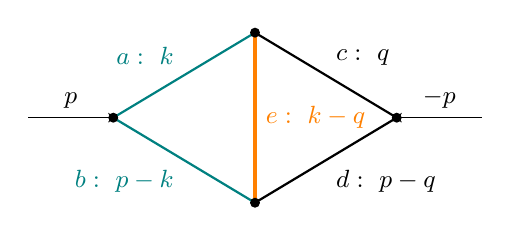
\begin{tikzpicture}[scale=.9, every node/.style={font=\small}]
\coordinate (L) at (0,0);\coordinate (R) at (4,0);
\coordinate (T) at (2,1.2);\coordinate (B) at (2,-1.2);
\draw[thick,teal] (L)--node[above left]{$a:\ k$}(T);
\draw[thick,teal] (L)--node[below left]{$b:\ p-k$}(B);
\draw[thick] (R)--node[above right]{$c:\ q$}(T);
\draw[thick] (R)--node[below right]{$d:\ p-q$}(B);
\draw[very thick,orange] (T)--node[right]{$e:\ k-q$}(B);
\draw[->] (-1.2,0)--node[above]{$p$}(L);
\draw[<-] (R)--node[above]{$-p$}(5.2,0);
\foreach \x in {L,R,T,B}{\fill (\x) circle (2pt);}
\end{tikzpicture}
\end{center}
两个三角形 $\{a,b,e\}$ 与 $\{c,d,e\}$ 共享中央边；整体有 $V=4$、$I=5$、$L=2$、$\omega=2$，两个子图各有 $\omega_\gamma=0$。固定标签的图权重为 $1/S=1/2$。

\paragraph{先读结果与约定。}
记 $M=m^2>0$、$s=p_E^2$，两次积分测度为 $d^6k/\pi^3$ 与 $d^6q/\pi^3$。在 $s=M=1$，未乘图权重与耦合的有限结果为
\[
 \boxed{J_R(1,1)\simeq +0.00277755520593736.}
\]
乘图权重后是约 $0.00138877760296868$；若使用通常的每圈 $d^6k/(2\pi)^6$，另有 $(4\pi)^{-6}$。有效作用量的整体符号及耦合约定仍须单列。

\paragraph{论证链。}
先在正则化传播子上执行子图零阶减除，再执行整体二阶减除；Gauss 积分与总 Schwinger 尺度积分将结果化为四维参数积分。只在相消组合上建立控制函数，避免把发散项分开积分。随后独立分析单硬圈、可比双硬圈与软差动量通道，证明动量空间绝对收敛。两条控制收敛论证将两种表示连接起来。下面的英文正式推导给出全部常数；后面的中文数值部分将它们对应到实际程序。
\clearpage
\tableofcontents
\clearpage
\section{Recursive BPH subtraction of the overlapping two-loop graph}
We consider one particular massive Euclidean six-dimensional graph, rather
than infer a general BPH theorem from a finite computation. Write
\[
 D(r)=\frac1{r^2+M},\qquad M=m^2>0,\qquad s=p^2\geq0,
 \qquad d\mu(k)=\frac{d^6k}{\pi^3}.
\]
The unweighted integral has integrand
\[
 I=D(k)D(p-k)D(q)D(p-q)D(k-q).
\]
The two proper divergent subgraphs are the overlapping triangles
\(\gamma_1=\{a,b,e\}\) and \(\gamma_2=\{c,d,e\}\), each of Taylor degree zero.
The graph itself has Taylor degree two. Bogoliubov's recursion gives
\begin{align}
 \bar R I&=I-T_1I-T_2I,\\
 T_1I&=D(k)^3D(q)D(p-q),&
 T_2I&=D(q)^3D(k)D(p-k),\\
 RI&=(1-t_G^2)\bar R I.
\end{align}
The independent external inputs of the first triangle are \((q,p)\); its
loop momentum \(k\) is held fixed by \(T_1\). The second operation is symmetric.
The two triangles cannot belong to one disjoint spinney, so there is no
\(T_1T_2\) product. Expanding the recursion produces six terms, but none is
to be integrated separately without a common regulator.

\subsection{A common regulator and the finite parameter representation}
For every original edge use
\[
 D_\eta(r)=\int_\eta^\infty e^{-\alpha(r^2+M)}\,d\alpha,
 \qquad\eta>0.
\]
Apply the subgraph and overall Taylor operations to the regulated propagators
before Gaussian integration. Counterterms retain all five original Schwinger
labels, so the integration domain \(\alpha_e\geq\eta\) is common to all terms.
In the order \(D(k),D(p-k),D(q),D(p-q),D(k-q)\), call these labels
\(a,b,c,d,e\). Gaussian integration gives
\begin{align}
 U&=(a+b)(c+d)+e(a+b+c+d),\\
 V&=ab(c+d)+cd(a+b)+e(a+c)(b+d),&w&=V/U,\\
 U_1&=(a+b+e)(c+d),&w_1&=cd/(c+d),\\
 U_2&=(a+b)(c+d+e),&w_2&=ab/(a+b).
\end{align}
Set \(\alpha_e=\rho x_e\), \(\sum x_e=1\). The five-parameter measure
contributes \(\rho^4\), while the two-loop Gaussian contributes
\(\rho^{-6}\). The overall subtraction replaces \(e^{-s\rho w}\) by
\(e^{-s\rho w}-1+s\rho w\). Its common radial lower limit is
\(T(x)=\eta/\min_e x_e\). Define
\begin{align}
 K_T(z)&=\int_T^\infty\rho^{-2}e^{-M\rho}
              (e^{-z\rho}-1+z\rho)\,d\rho,\\
 K(z)=K_0(z)&=(M+z)\log(1+z/M)-z.
\end{align}
Uniformly for all \(T\geq0\) and \(z\geq0\),
\begin{equation}\label{eq:kernel-bounds}
 0\leq K_T(z)\leq\frac{z^2}{2M},\qquad
 0\leq K_T'(z)\leq\log(1+z/M)\leq\frac zM,\qquad
 0\leq K_T''(z)\leq\frac1{M+z}.
\end{equation}
These inequalities will provide a regulator-independent integrable majorant;
the limit \(\eta\downarrow0\) will therefore follow from dominated convergence.

On the simplex write
\[
 a=Au,\quad b=A(1-u),\quad c=Bv,\quad d=B(1-v),\quad e=E,
 \qquad A+B+E=1.
\]
The Jacobian is \(AB\,dA\,dB\,du\,dv\), with \(u,v\in[0,1]\). Let
\(h(t)=t(1-t)\). Then
\begin{align}
 U&=AB+E(A+B),& U_1&=B(A+E),& U_2&=A(B+E),\\
 x&=Ah(u),& y&=Bh(v),& z&=\frac{EAB}{U}(u-v)^2,\\
 w&=x+y+z.&&&
\end{align}
The finite representation is
\begin{equation}\label{eq:finite-overlap}
 J_R(s,M)=\int_{A,B\geq0,\ A+B\leq1}\!dA\,dB
       \int_0^1du\int_0^1dv\;AB\,H,
 \quad
 H=\frac{K(sw)}{U^3}-\frac{K(sy)}{U_1^3}-\frac{K(sx)}{U_2^3}.
\end{equation}
No symmetry weight, coupling, or \((4\pi)^{-6}\) loop-measure factor is
included in \(J_R\).

\subsection{An explicit absolute majorant for every parameter UV face}
Because \(EAB/U\leq AB/(A+B)\), the weighted variance identity implies
\[
 0\leq w\leq\frac{A+B}{4}.
\]
On the half-domain \(A\leq B\),
\[
 0\leq w-y\leq A,
\]
since \(z/A\leq(u-v)^2\) and \(h(u)+(u-v)^2\leq1\).
Pair the bare contribution with the first counterterm on this half-domain.
With \(r=A+E\), \(U=U_1+AE\), so
\[
 0\leq U_1^{-3}-U^{-3}\leq3AE/U_1^4.
\]
Using the mean value theorem and \eqref{eq:kernel-bounds} gives
\begin{equation}\label{eq:majorant}
 AB|H|\leq\frac{s^2}{M}(\mathcal B_1+\mathcal B_2+\mathcal B_3),
\end{equation}
where
\[
 \mathcal B_1=\frac{A^2(A+B)}{4B^2(A+E)^3},\qquad
 \mathcal B_2=\frac{3A^2E}{32B(A+E)^4},\qquad
 \mathcal B_3=\frac{B}{32(B+E)^3}.
\]
The \(u,v\) intervals have unit volume. To integrate the remaining two
parameters, set \(A=rt\), \(E=r(1-t)\), \(B=1-r\). The upper limit of
\(t\) is \(\min(1,(1-r)/r)\). Direct antiderivatives give
\begin{align}
 \int_{A\leq B}\mathcal B_1\,dA\,dB&=\frac{\log2}{6}-\frac1{96},\\
 \int_{A\leq B}\mathcal B_2\,dA\,dB&=\frac{\log2}{16}-\frac9{256},\\
 \int_{A\leq B}\mathcal B_3\,dA\,dB&=\frac1{128}.
\end{align}
The other half-domain follows by exchanging the loops. Consequently
\begin{equation}\label{eq:quadratic-bound}
 \int AB|H|\leq C\frac{s^2}{M},\qquad
 C=\frac{11\log2}{24}-\frac{29}{384}
   =0.242171624423308\ldots.
\end{equation}
This explicitly controls the triangle UV faces, their adjacent corners and
the overall radial limit. It is not just superficial power counting.

The same majorant also controls the Gaussian-integrated Schwinger expression
before radial integration: write the bare-minus-counterterm pair as
\[
 U^{-3}[E_\rho(sw)-E_\rho(sy)]
 -(U_1^{-3}-U^{-3})E_\rho(sy),\qquad
 E_\rho(z)=e^{-\rho z}-1+\rho z.
\]
The first bracket, inverse-cube difference, and \(E_\rho\) are nonnegative.
Take the triangle inequality first, and then integrate each positive piece
radially. They produce exactly the \(K\)-differences and \(K\)-values above.
Thus absolute control does not depend on cancellation after the radial
integral has already been performed.

\subsection{Uniform external-scale and derivative bounds}
For large external momentum a purely quadratic bound in \(s\) is unnecessarily
weak. Let \(L=\log(1+s/(4M))\). Use \(K'\leq L\) and
\(K(sy)\leq sBL/4\) in the same pair. The two resulting half-domain integrals
are respectively \(1/2\) and \(1/8\), so their sum contributes at most
\(5sL/8\). The remaining counterterm obeys
\[
 \int_0^{1/2}\frac{K(sA/4)}{A^2}\,dA
 \leq\frac s4\left(\ell+\frac{\ell^2}{2}\right),\qquad
 \ell=\log(1+s/(8M))\leq L.
\]
For example, integrate by parts and use
\[
 \int_0^T\frac{\log(1+t)}t\,dt
 \leq\log(1+T)+\frac12\log^2(1+T).
\]
The derivative of the right side minus the left side is nonnegative because
\(\log(1+T)\leq T\). Reflecting both half-domains yields
\begin{equation}\label{eq:global-bound}
 |J_R|\leq\int AB|H|
 \leq\min\left\{\frac{Cs^2}{M},\quad
          s\left(\frac74L+\frac14L^2\right)\right\}.
\end{equation}
Thus the global growth is at most \(s\log^2s\). For \(|p|\leq P\) and
\(m^2\geq m_0^2>0\), replacing \(s\) by \(P^2\) and \(M\) by \(m_0^2\)
gives a compact-uniform bound.

Differentiation under the parameter integral is justified by replacing
\(K(sw)\) with \(w\log(1+sw/M)\) or \(w^2/(M+sw)\) and repeating the
same majorant argument. For \(s>0\),
\begin{align}
 |J_R'(s)|&\leq\min\left\{2Cs/M,\quad1+7L/4+L^2/4\right\},\\
 |J_R''(s)|&\leq\min\left\{2C/M,\quad(5/4+L/2)/s\right\}.
\end{align}
At \(s=0\), use the continuous bound \(2C/M\); also
\(J_R(0)=J_R'(0)=0\). In vector momentum variables,
\[
 |\nabla_p J_R|\leq4CP^3/m_0^2,\qquad
 \|\nabla_p^2J_R\|\leq12CP^2/m_0^2
 \quad (|p|\leq P,\ m^2\geq m_0^2).
\]

\subsection{A separate momentum-space absolute-convergence proof}
The parameter \(L^1\) norm need not equal the momentum \(L^1\) norm.
We therefore prove absolute convergence of the original twelve-dimensional
subtracted expression independently. Write
\(\langle r\rangle=\sqrt{r^2+m^2}\). For a unit direction,
\[
 |\partial^nD(r)|\leq c_n\langle r\rangle^{-2-n},\qquad
 (c_0,c_1,c_2,c_3)=(1,2,10,72).
\]
Taylor's integral remainder applied to \(\bar R I\) gives \(P^3/6\) times
a supremum of its third directional derivative for \(|p|\leq P\).

First consider \(|k|\geq2(|q|+P+m)\). Put
\(h=D(k)D(k-p)D(k-q)\), \(a_q=D(q)D(q-p)\), and
\(\Lambda=1+P/m\). Pair before estimating:
\[
 \bar R I=(h-D(k)^3)a_q-D(q)^3D(k)D(k-p).
\]
The mean value theorem, shifted-bracket comparison, and the derivative bounds
give
\begin{align}
 |h-D(k)^3|&\leq64(P+|q|)\langle k\rangle^{-7},\\
 |\partial^nh|&\leq(64,640,9216)_n\langle k\rangle^{-6-n},
       && n=1,2,3,\\
 |\partial^ja_q|&\leq c_j\Lambda^{2+j}\langle q\rangle^{-4-j}.
\end{align}
Leibniz's formula then yields
\[
 |RI|\leq\frac{P^3C_h(\Lambda)}6
        \langle k\rangle^{-7}\langle q\rangle^{-6},
 \quad
 C_h(\Lambda)=4608\Lambda^6+1920\Lambda^4+3840\Lambda^3
                  +9216\Lambda^2+2304.
\]
The normalized radial angular factor is one, and
\[
 \int_{|k|\geq2(|q|+P+m)}\langle k\rangle^{-7}\,d\mu(k)
 \leq\frac1{2\langle q\rangle},\qquad
 \int\langle q\rangle^{-7}\,d\mu(q)=\frac8{15m}.
\]
Both symmetric hierarchy regions together therefore have absolute integral
at most
\[\frac{4C_h(\Lambda)P^3}{45m}.\]

Outside these regions, let \(K=\max(|k|,|q|)\geq K_0=8(P+m)\).
Then both loop momenta are at least \(K/4\), and their external shifts at
least \(K/8\). After three derivatives, the bare term is bounded by
\(264\,8^{11}K^{-11}D(k-q)\), and both counterterms together by
\(144\,8^{13}K^{-13}\). This does not assume that \(k-q\) is hard.
On a dyadic shell \(K\in[K_n,2K_n]\), \(K_n=2^nK_0\),
\[
 \int_{|k-q|\leq4K_n}D(k-q)\,d\mu(q)\leq64K_n^4,
 \qquad\operatorname{vol}\{|k|\leq2K_n\}=\frac{64K_n^6}{6}.
\]
The shell integrals are thus bounded by constants times \(P^3/K_n\), whose
sum is finite. One explicit bound for this comparable region is
\[
 \frac{P^3}{3K_0}
 \left[264\,8^{11}\frac{2048}{3}
              +144\,8^{13}\frac{1024}{9}\right].
\]
Finally \(K\leq K_0\) is compact. The third derivative is bounded by
\(408m^{-13}\), so \(|RI|\leq68P^3m^{-13}\); the product-ball volume is
\(K_0^{12}/36\). These three regions prove a finite momentum \(L^1\) norm.
They also give uniform control for \(|p|\leq P\), \(m\geq m_0>0\).

The same estimates hold uniformly for \(D_\eta\). Indeed, after differentiating
its Schwinger representation, the absolute values of the positive
\(\alpha\)-moment contributions from \(\eta\) to infinity are bounded by
their integrals from zero to infinity, giving the same constants
\(1,2,10,72\). The propagator-difference estimates are uniform as well.
Momentum-space dominated convergence proves
\(\int RI_\eta\to\int RI_0\); parameter-space dominated convergence proves
that the same limit is \eqref{eq:finite-overlap}. This establishes their
equality without a termwise exchange of unregulated divergent integrals.

\subsection{Interpretation}
The bounds concern this graph with a common positive mass. The explicit constant
\(C\) controls the parameter norm and amplitude magnitude; the separate,
much rougher momentum \(L^1\) estimate has different constants. Neither is a
quadrature error estimate. At \(s=M=1\), the computed benchmark is approximately
\(J_R=0.00277755520593736\); multiplying only the graph weight \(1/S=1/2\)
halves it. Couplings, standard loop-measure factors and any effective-action
sign convention remain separate. The construction follows the recursive
framework of Kennedy's BPH treatment; it does not establish a general
arbitrary-loop theorem from this representative example.


\clearpage
\section{数值算法：把紫外相消写成有界积分核}
\subsection{先消去最容易出错的相消}
利用 $k\leftrightarrow q$ 对称性限制 $A\leq B$ 并乘 $2$，采用射影尺度 $B=1$，写 $A=X\in[0,1]$、$E=Z\in[0,\infty)$。本节只说明换元，$M$ 仍表示质量平方。径向质量参数变为 $M(1+X+Z)$，不能误写成固定 $M$。
令 $Z=Xr/(1-r)$、$W=1-r$，则对数紫外面 $X,Z\to0$ 的首项相消可用恒等式
\[
 K_M(y+h)-K_M(y)
 =h\log(1+y/M)+K_{M+y}(h)
\]
精确处理。这里 $K_M(z)=(M+z)\log(1+z/M)-z$；求差时没有用两个几乎相等的浮点数直接相减。
定义连续函数
\[
 \mathfrak h(z)=\frac{(1+z)\log(1+z)-z}{z^2}
  =\int_0^1\frac{1-v}{1+zv}\,dv,\qquad \mathfrak h(0)=\frac12.
\]
在小 $z$ 时用其收敛级数计算，另把 $\sigma^2=(s/M)^2$ 解析提取，最终计算 $J_R=(s(s/M))G(s/M)$，避免先平方很小的比值造成下溢。

\subsection{实际采用的两张有界参数图}
在 $(X,W)$ 单位正方形分别取
\[
 (X,W)=(t,ty),\qquad (X,W)=(ty,t),
 \qquad 0\leq t,y\leq1,
\]
两张图的 Jacobian 均为 $t$。记
\[
 r=1-W,\quad C=1+Xr,\quad d=1+y-ty\geq1,
 \quad A_u=u(1-u),\quad B_v=v(1-v),
\]
\[
 T=A_u+\frac{r(u-v)^2}{C},\qquad
 \nu=\frac{W}{X+W}
 =\begin{cases}y/(1+y),&\text{第一张图},\\1/(1+y),&\text{第二张图},\end{cases}
 \qquad\nu_*=\frac{\nu}{1+\sigma B_v\nu}.
\]
令 $\ell(z)=\log(1+z)/z$，$\ell(0)=1$。程序中去除 $\sigma^2$ 后的有界核为
\begin{align}
 F={}&\frac{2tW}{C^3}\biggl[
 T B_v\nu\,\ell(\sigma B_v\nu)
 +XT^2\nu_*\mathfrak h(\sigma XT\nu_*)\notag\\
 &\hspace{23mm}-r(3+3Xr+X^2r^2)B_v^2\nu\,
                    \mathfrak h(\sigma B_v\nu)\biggr]\notag\\
 &-\frac{2y\nu}{d^3}A_u^2\mathfrak h(\sigma X A_u\nu),\\
 J_R(s,M)={}&\frac{s^2}{M}\sum_{j=1}^2\int_{[0,1]^4}F_j(t,y,u,v;\sigma)\,dt\,dy\,du\,dv.
\end{align}
所有分母都有明确的正下界，$t=0$ 等边界可连续取值。对零外动量返回精确的 $0$。标准库实现逐维使用 Gauss--Legendre 求积；默认每维 $16$ 阶，总节点数 $2\times16^4$。程序分别记录两个阶数的值、差值与耗时，不能把差值误标为严格误差上界。

\subsection{真正独立的复算路线}
独立工具保留 $B=1$ 的射影坐标，把区域分为 $E=A y$、$A=E y$ 与 $E\geq1$ 的三张图。更重要的是，它不调用上面的对数核，而采用
\[
 K_M(sf)=s^2\int_0^1\frac{(1-r)f^2}{M+rsf}\,dr
\]
增加第五维积分。因此坐标和积分核都不同。可选 NumPy 环境只提供节点及数组运算；核心工作台依然只需要 Python 标准库。
\begin{center}
\begin{tabular}{ccc}
\toprule
$s/M$ & 独立五维结果（$M=1$） & 与四维核心的差（20 阶）\\
\midrule
0.1 & $0.00003559910372634172$ & $9.49\times10^{-20}$\\
1 & $0.002777555205937361$ & $4.34\times10^{-18}$\\
4 & $0.01675339249830868$ & $1.28\times10^{-16}$\\
\bottomrule
\end{tabular}
\end{center}
表中记录一次独立运行，最终源码版本的原始数据写在软件的 \path{results/overlap_comparison.json}。阶数变化与路线一致支持这些近似数值，但不提供严格的数字包围区间。上面的解析界解决收敛与尺度控制，不能当作此表的误差条。

\section{软件中的使用、验证与范围}
双击 Mac 的\texttt{启动分析.command}或 Windows 的\texttt{启动分析.bat}，将先重新生成报告，再打开本地计算工作台。在页面中输入 $p^2$、质量平方与积分阶数即可计算；保持启动窗口开启。直接打开 HTML 也能离线阅读预生成结果。使用说明和 JSON 保留所有归一化信息。
\begin{quote}\ttfamily\small
python3 -m phi3lab overlap --s 1 --m2 1 --order 16\par
python3 tools/verify\_tests.py\par
python tools/compare\_overlap.py
\end{quote}
最后一个命令在安装了 NumPy 的可选环境中执行。输入错误、非正质量、非有限数或超出支持阶数会明确报错。构建清单将源码指纹、输出文件与独立核查分开记录；源码改变后，旧的外部核查不会被重建报告冒充为当前证据。

本交付包含这张重叠图的减除、有限积分、解析界和可复算软件；图集共十三张；其余条目提供精确拓扑、权重、子图、递归展开与参数多项式。没有把这一个例子的结果外推为所有图的积分、所有圈数的 BPH 定理或 MS 与本方案的有限转换。

\section*{来源与工作归属}
方法主线参照 A. D. Kennedy, \emph{A Simple Proof of the BPH Theorem}, arXiv:hep-th/9612113，尤其第 3--5 节。现代 $\phi^3$ 与积分工具文献、版本和许可记录在软件的现代调研页。上述代表图的推导、算法、代码与复算在本次协作中完成；学生在项目报告中仍应据实区分自己掌握并复写的推导、软件辅助和未完成的一般论证。
\end{document}
